%%%%%%%%%%%%%%%%%%%%%%%%%%%%%%%%%%%%%%%%%
% Short Sectioned Assignment LaTeX Template Version 1.0 (5/5/12)
% This template has been downloaded from: http://www.LaTeXTemplates.com
% Original author:  Frits Wenneker (http://www.howtotex.com)
% License: CC BY-NC-SA 3.0 (http://creativecommons.org/licenses/by-nc-sa/3.0/)
%%%%%%%%%%%%%%%%%%%%%%%%%%%%%%%%%%%%%%%%%

%----------------------------------------------------------------------------------------
%	PACKAGES AND OTHER DOCUMENT CONFIGURATIONS
%----------------------------------------------------------------------------------------

\documentclass[paper=a4, fontsize=11pt]{scrartcl} % A4 paper and 11pt font size

% ---- Entrada y salida de texto -----

\usepackage[T1]{fontenc} % Use 8-bit encoding that has 256 glyphs
\usepackage[utf8]{inputenc}
%\usepackage{fourier} % Use the Adobe Utopia font for the document - comment this line to return to the LaTeX default

\usepackage{eurosym}
\usepackage{multirow}
% ---- Idioma --------

\usepackage[spanish, es-tabla]{babel} % Selecciona el español para palabras introducidas automáticamente, p.ej. "septiembre" en la fecha y especifica que se use la palabra Tabla en vez de Cuadro

% ---- Otros paquetes ----

\usepackage{url} % ,href} %para incluir URLs e hipervínculos dentro del texto (aunque hay que instalar href)
\usepackage{amsmath,amsfonts,amsthm} % Math packages
%\usepackage{graphics,graphicx, floatrow} %para incluir imágenes y notas en las imágenes
\usepackage{graphics,graphicx, float} %para incluir imágenes y colocarlas

% Para hacer tablas comlejas
%\usepackage{multirow}
%\usepackage{threeparttable}

%\usepackage{sectsty} % Allows customizing section commands
%\allsectionsfont{\centering \normalfont\scshape} % Make all sections centered, the default font and small caps

\usepackage{fancyhdr} % Custom headers and footers
\pagestyle{fancyplain} % Makes all pages in the document conform to the custom headers and footers
\fancyhead{} % No page header - if you want one, create it in the same way as the footers below
\fancyfoot[L]{} % Empty left footer
\fancyfoot[C]{} % Empty center footer
\fancyfoot[R]{\thepage} % Page numbering for right footer
\renewcommand{\headrulewidth}{0pt} % Remove header underlines
\renewcommand{\footrulewidth}{0pt} % Remove footer underlines
\setlength{\headheight}{13.6pt} % Customize the height of the header

\numberwithin{equation}{section} % Number equations within sections (i.e. 1.1, 1.2, 2.1, 2.2 instead of 1, 2, 3, 4)
\numberwithin{figure}{section} % Number figures within sections (i.e. 1.1, 1.2, 2.1, 2.2 instead of 1, 2, 3, 4)
\numberwithin{table}{section} % Number tables within sections (i.e. 1.1, 1.2, 2.1, 2.2 instead of 1, 2, 3, 4)

\setlength\parindent{0pt} % Removes all indentation from paragraphs - comment this line for an assignment with lots of text

\newcommand{\horrule}[1]{\rule{\linewidth}{#1}} % Create horizontal rule command with 1 argument of height



%----------------------------------------------------------------------------------------
%	TÍTULO Y DATOS DEL ALUMNO
%----------------------------------------------------------------------------------------

\title{	
\normalfont \normalsize 
\textsc{\textbf{Ingeniería de Servidores (2016-2017)} \\ Grado en Ingeniería Informática \\ Universidad de Granada} \\ [25pt] % Your university, school and/or department name(s)
\horrule{0.5pt} \\[0.4cm] % Thin top horizontal rule
\huge Memoria Práctica 1 \\ % The assignment title
\horrule{2pt} \\[0.5cm] % Thick bottom horizontal rule
}

\author{David Criado Ramón} % Nombre y apellidos

\date{\normalsize\today} % Incluye la fecha actual

%----------------------------------------------------------------------------------------
% DOCUMENTO
%----------------------------------------------------------------------------------------

\begin{document}

\maketitle % Muestra el Título

\newpage %inserta un salto de página

\tableofcontents % para generar el índice de contenidos

\listoffigures

\listoftables

\newpage

%----------------------------------------------------------------------------------------
%	Cuestión 1
%----------------------------------------------------------------------------------------

\section{¿Qué modos y/o tipos de ``virtualización'' existen?}
Existen 3 tipos de virtualización \cite{c1-1}
\begin{itemize}
	\item \textbf{Virtualización completa} - Consiste en la mezcla de emulación vía software de aquellas instrucciones que puedan afectar al buen funcionamiento del sistema y ejecución directa sobre el hardware de las que no traduciéndolas en binario de un sistema a otro.
	
	\item \textbf{Virtualización con un host} - El sistema host (sobre el que se instala el software de virtualización) actúa como capa intermedia entre hardware y el sistema que es virtualizado.
	
	\item \textbf{Paravirtualización} - El sistema operativo  virtualizado es modificado para conseguir que la ejecución se realice en el procesador sin necesidad de traducción.
\end{itemize}


%----------------------------------------------------------------------------------------
%	Cuestión 2
%----------------------------------------------------------------------------------------

\section{Muestre los precios y características de varios proovedores de VPS (Virtual Private Server) y compare con el precio de servidores dedicados (administrados y no administrados). Comente diferencias.}

\begin{itemize}
	\item ARSYS
	\begin{itemize}
		\item VPS - 10 \euro/mes CentOS | Ubuntu | Debian con 40 GB SSD, 1 GB RAM, transferencia ilimitada, 1 procesador vCPU Intel Xeon.\cite{c2-1}
		\item Dedicado - 125 \euro/mes con Intel Xeon 4 Core 2 Ghz, 8 GB RAM, 2x500 GB SATA RAID1, transferencia ilimitada.\cite{c2-2}
	\end{itemize}
	\item HOSTALIA
	\begin{itemize}
		\item VPS - 11,21 \euro/mes, CentOS con 25 GB disco, 1 GB RAM, 1000 GB transferencia,  2 procesadores Intel Xeon.\cite{c2-3}
		\item Dedicado - 99,90 \euro/mes (6 primeros meses 69,90 \euro) con Intel Xeon E3-1230 v5, 16 GB RAM, 2 x 1TB SATA, transferencia ilimitada.\cite{c2-4}
	\end{itemize}
	\item UNELINK
	\begin{itemize}
		\item VPS - 12,09 \euro/mes, con Intel Xeon 3,20 GHz, 50 GB disco, 1 GB RAM DDR3, transferencia ilimitada.\cite{c2-5}
		\item Dedicado - 59,83 \euro/mes con Intel Processor C2550 4 núcleos 2.40 GHz, 4 GB RAM, 500 GB disco, transferencia ilimitada.\cite{c2-6}
	\end{itemize}
\end{itemize}
\textit{Nota: Se han cogido todas las opciones de menor coste.}\\
Los VPS nos ofrecen compartir el hardware para varios clientes. Por tanto, su coste es considerablemente más barato ya que disfrutamos de muchas menos prestaciones y, en mi opinión, son los más indicados para pequeños servidores.

Los servidores dedicados nos dan el control de todo el hardware de la máquina por lo que ganamos muchas prestaciones pero a cambio de un precio considerable.

%----------------------------------------------------------------------------------------
%	Cuestión 3
%----------------------------------------------------------------------------------------
\section{Enumere y explique brevemente al menos tres de las innovaciones en Windows Server 2016 y 2012 R2 respecto a 2008R2. ¿Qué es Windows Server 2016 nano?}

\subsection{Enumere y explique brevemente al menos tres de las innovaciones en Windows Server 2016 y 2012 R2 respecto a 2008R2.}
Entre las diferencias que encontramos \cite{c3a} podemos describir:
\begin{itemize}
	\item \textbf{QoS de almacenamiento para Hyper-V} - Permite limitar e informar el número de operaciones  de entrada/salida que están ocurriendo a cada usuario según nos interese.\cite{c3a1}
	\item \textbf{Migración de almacenamiento en vivo} - Permite trasladar los datos de varios servidores Hyper-V mientras siguen completamente operativos.\cite{c3a2}
	\item \textbf{Control de acceso dinámico} - \textit{``Permite controlar quién accede a la información y auditar quién ha accedido a ella''}\cite{c3a3}
	
\end{itemize}
\subsection{¿Qué es Windows Server 2016 nano?}
Es una opción de instalación de Windows Server 2016 todavía más pequeña que ``Core''. No tiene ningún tipo de GUI o terminal local, por lo que sólo se puede controlar con acceso remoto y solo soporta aplicaciones de 64-bits.\cite{c3b}

%----------------------------------------------------------------------------------------
%	Cuestión 4
%----------------------------------------------------------------------------------------

\section{¿Qué son los productos MAAS y Landscape ofrecidos por Canonical(la empresa que desarrolla Ubuntu)?}
\subsection{MAAS}
\textit{``MAAS nos permite manejar servidores físicos como si fuesen máquinas virtuales en la nube''}\cite{c4a}. En los servidores que se encuentren en MAAS podemos instalar sistemas operativos dinámicamente (están soportados Ubuntu, CentOS y Windows), configurar sus interfaces de red y de almacenamiento  y encenderlos y apagarlos acorde con la demanda que tengamos en cada momento \cite{c4a1}
\subsection{Landscape}
Landscape permite administrar una gran cantidad de ordenadores Ubuntu Desktop, Server o en la nube. Esta herramienta nos permite monitorizar todos los dispositivos conectados, actualizar todas las máquinas, crear nuestros propios repositorios y administrar usuarios y permisos entre otros. \cite{c4b}
%----------------------------------------------------------------------------------------
%	Cuestión 5
%----------------------------------------------------------------------------------------
\section{¿Qué relación tiene CentOS con Red Hat y con el proyecto Fedora?}
El proyecto Fedora nació al dividir Red Hat Linux en Red Hat Enterprise Linux (versión comercial, no gratuita) y el proyecto Fedora (gratuito y dónde se suelen añadir la mayoría de las novedades creadas por la comunidad). Así pues el proyecto Fedora, es en el que se basan las nuevas versiones de Red Hat Enterprise Linux.

CentOS, es un sistema operativo que deriva de Red Hat Entrepise Linux y otras soluciones de software libre, facilitando el uso de software libre, siendo gratuito y relativamente estable.\cite{c5}
%----------------------------------------------------------------------------------------
%	Cuestión 6
%----------------------------------------------------------------------------------------
\section{¿Qué diferencias hay entre RAID mediante SW y mediante HW?}
El RAID software ``\textit{suele ser más barato, esto se debe a que es un RAID a nivel de sistema operativo y depende la memoria y la CPU del host}''. El RAID hardware ``\textit{tiene en un su controlador una CPU y memorias caché dedicada y una batería de reserva y no depende del sistema host}''\cite{c6}
%----------------------------------------------------------------------------------------
%	Cuestión 7
%----------------------------------------------------------------------------------------
\section{¿Qué es LVM? ¿Qué ventaja tiene para un servidor de gama baja? Si va a tener un servidor web, ¿le daría un tamaño grande o pequeño a /var?}

\subsection{¿Qué es LVM?}
``LVM es una herramienta para la gestión de discos que incluye la asignación, striping, reflejamiento y cambio de tamaño de los volúmenes lógicos''\cite{c7a}
\subsection{¿Qué ventaja tiene para un servidor de gama baja?}
En un servidor de gama baja nos permite añadir nuevos volúmenes lógicos, modificar el tamaño de estos o eliminarlos de manera fácil y sin necesidad de apagar el sistema operativo, por lo que podemos adaptarnos con facilidad a las necesidad de uso de disco de cada uno de los clientes.\cite{c7b}
\subsection{Si va a tener un servidor web, ¿le daría un tamaño grande o pequeño a /var?}
Grande, porque en la mayoría de servidores web la ubicación por defecto que se asigna al directorio dónde se guardan los archivos de la páginas web es, como con el servidor HTTP Apache es \textit{/var/www}.
%----------------------------------------------------------------------------------------
%	Cuestión 8
%----------------------------------------------------------------------------------------
\section{¿Debemos cifrar también el volumen que contiene el espacio para swap? ¿y el volumen en el que montaremos /boot?}
 
\subsection{¿Debemos cifrar también el volumen que contiene el espacio para swap?}
Sí deberíamos cifrarlo porque \textit{``si el sistema operativo decide que ha de pasar una página a disco y en el contenido de esta se encuentra una contraseña, dicho dato se encontrará desencriptado en nuestro disco duro.''} \cite{c8a}

\subsection{¿Y el volumen en el que montaremos /boot?}
Podríamos encriptarlo pero deberíamos de preparar alguna partición o dispositivo alternativo con la capacidad de desencriptar /boot para poder arrancar el sistema operativo.

%----------------------------------------------------------------------------------------
%	Cuestión 9
%----------------------------------------------------------------------------------------
\section{Imagine que tiene un disco con tecnología SSD ¿Qué puntos de montaje utilizaría para este? Justifique qué tipo de sistema de archivos utilizaría para tener un servidor de streaming.}

\subsection{Imagine que tiene un disco con tecnología SSD ¿Qué puntos de montaje utilizaría para este?}
Sería lógico poner todas los binarios en él (puntos de montaje: /bin y /usr/bin), root (/) y los archivos personales de los usuarios (/home).
\subsection{Justifique qué tipo de sistema de archivos utilizaría para tener un servidor de streaming?}
Utilizaría ext4 {\cite{c9b}, ya que, por ejemplo, retrasa la escrituras de los bloques y soluciona mejor los problemas de fragmentación, entre otros, que su mayor competidor (NTFS).
%----------------------------------------------------------------------------------------
%	Cuestión 10
%----------------------------------------------------------------------------------------
\section{Muestre como ha quedado particionado el disco una vez el sistema está instalado y ha iniciado sesión (comando: lsblk)}

\begin{figure}[H]
	\centering
		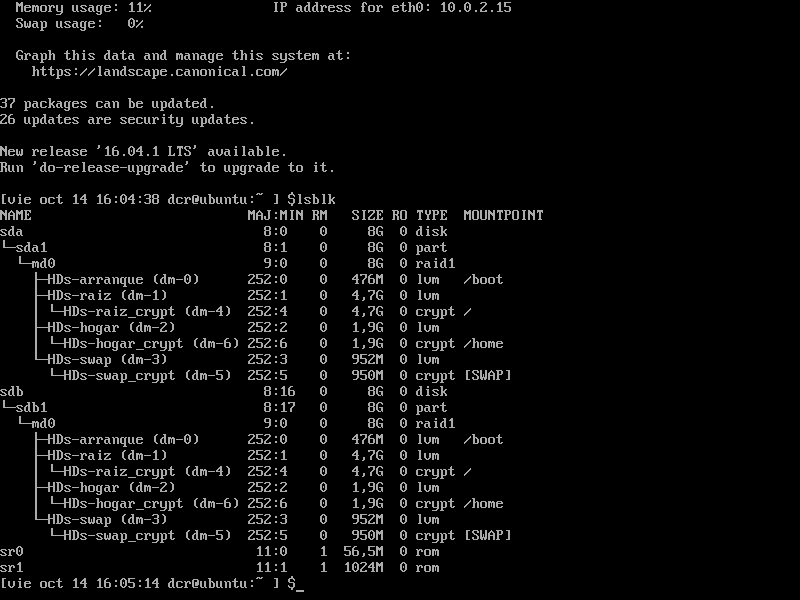
\includegraphics[width=1\textwidth]{lsblk.png}
		\caption{Captura de pantalla de lsblk tras instalar Ubuntu Server}
\end{figure}
%----------------------------------------------------------------------------------------
%	Cuestión 11
%----------------------------------------------------------------------------------------
\section{¿Cómo ha hecho el disco 2 ``arrancable''? ¿Qué hace el comando grub-install?}
\subsection{¿Cómo ha hecho el disco 2 ``arrancable``?}
Ejecutando el comando \textit{grub-install /dev/sdb}. \textit{Nota: así solo conseguimos que sea arrancable pero acabamos en una consola de recuperación}

\subsection{¿Qué hace el comando grub-install?}
Instala grub en el dispositivo indicado.\cite{c11-1} Grub es un gestor de arranque que soporta múltiples sistemas operativos y nos permite fácilmente seleccionar el que deseamos arrancar o si no lo reconoce o por otros motivos acceder a una consola que nos permita realizar el arranque manualmente. \cite{c11-2}
%----------------------------------------------------------------------------------------
%	Cuestión 12
%----------------------------------------------------------------------------------------

\section{¿Qué diferencia hay entre Windows Server Standard y Datacenter?}
Hasta la versión Windows Server 2012 R2 la principal diferencia entre ambos era que \textit{Standard} permitía sólo dos máquinas virtuales mientras que \textit{Datacenter} te otorgaba un número ilimitado de ellas.\cite{c12-1}  A partir de la versión Windows Server 2016, aparte de seguir manteniendo la diferencia previamente mencionada, se añaden nuevas características a la versión \textit{Datacenter} como, por ejemplo, ``Espacios de almacenamiento directo o máquinas virtuales blindadas'' \cite{c12-2}
%----------------------------------------------------------------------------------------
%	Cuestión 13
%----------------------------------------------------------------------------------------
\section{Continúe con el proceso de definición de RAID1 para los dos discos de 50 MiB que ha creado. Muestre el proceso con capturas de pantalla}
\begin{figure}[H]
	\centering
	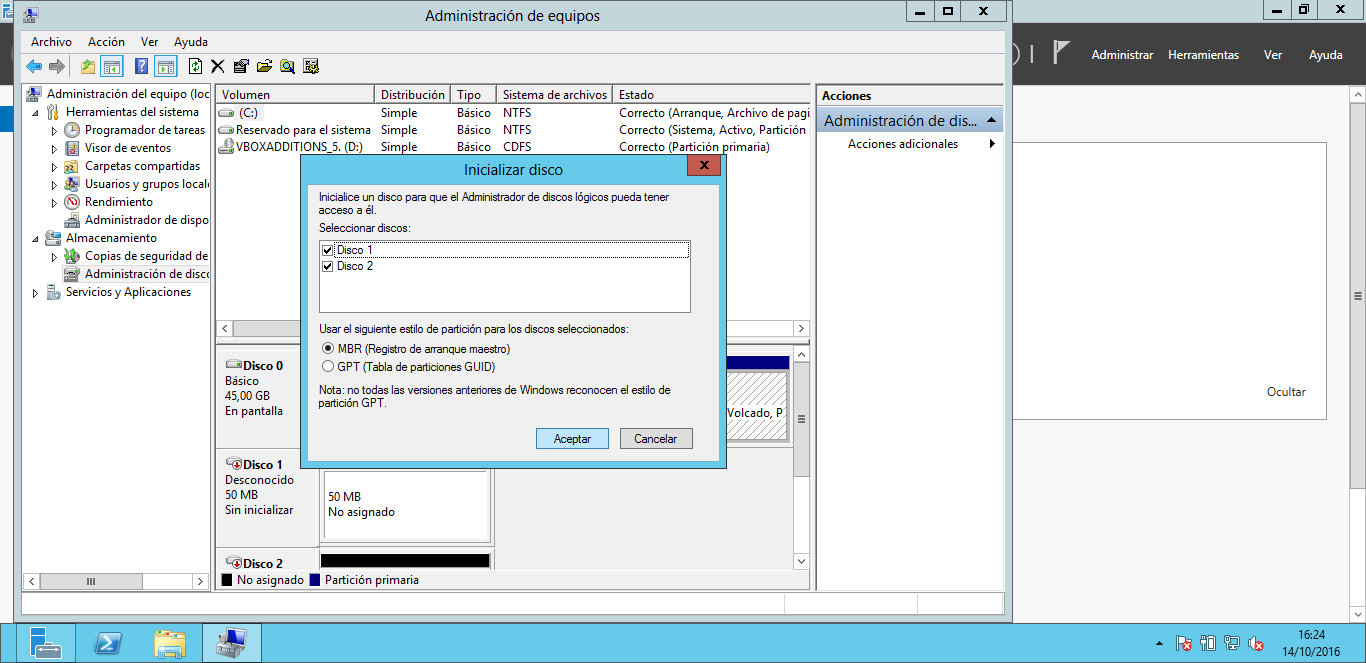
\includegraphics[width=0.9\textwidth]{raid1-1.png} 
	\caption{Tras reconocer los nuevos discos escogemos uno de los estilos de partición.}
\end{figure}

\begin{figure}[H]
	\centering
	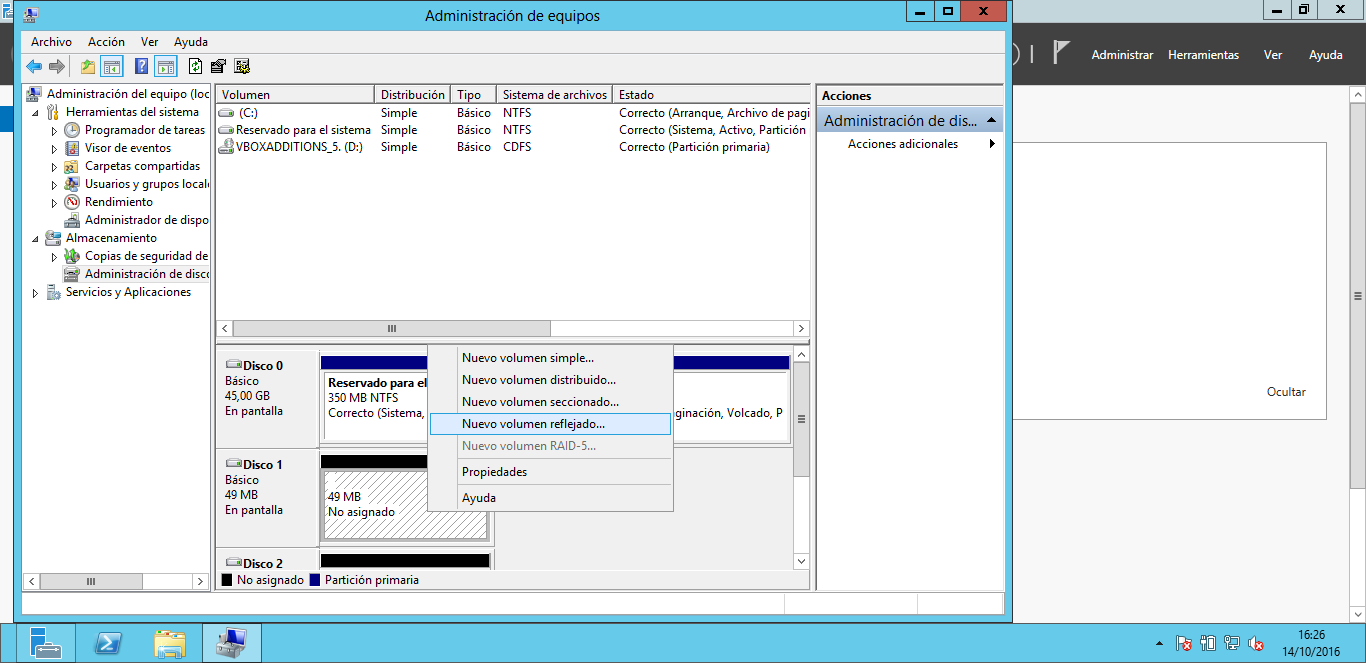
\includegraphics[width=0.9\textwidth]{raid1-2.png}
	\caption{Haciendo click derecho sobre uno de los nuevos discos escogemos ```Nuevo volumen reflejado...''}
\end{figure}
	
\begin{figure}[H]
	\centering
	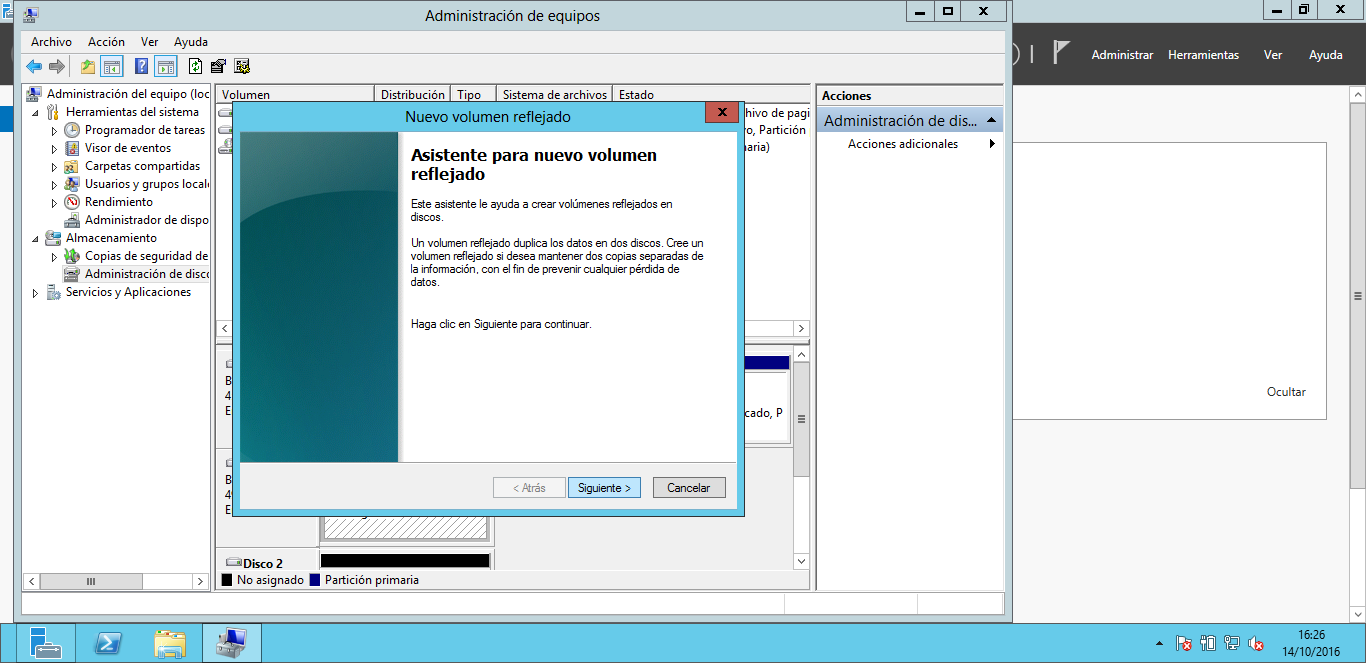
\includegraphics[width=0.9\textwidth]{raid1-3.png} 
	\caption{Se abre un asistente y pulsamos en siguiente.}
	
\end{figure}

\begin{figure}[H]
	\centering
	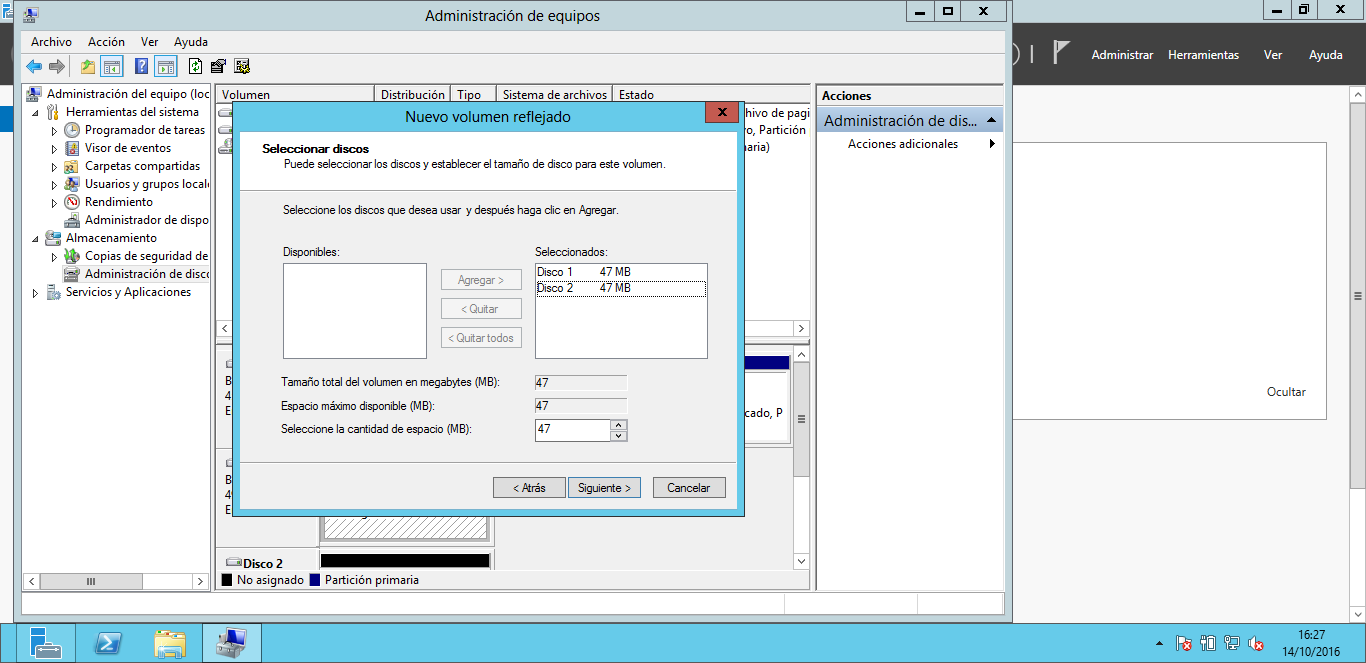
\includegraphics[width=0.9\textwidth]{raid1-4.png}
	\caption{Dejamos ambos discos como seleccionados y pulsamos en siguiente.}
\end{figure}

\begin{figure}[H]
	\centering
	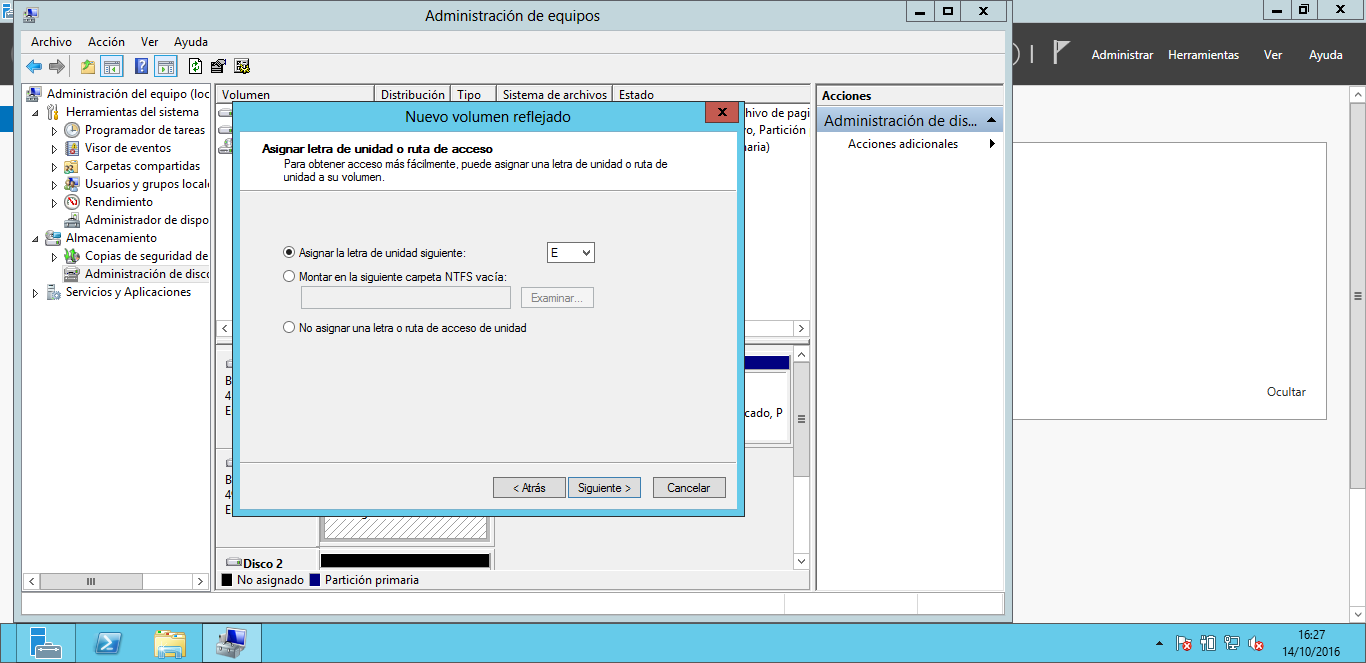
\includegraphics[width=0.9\textwidth]{raid1-5.png} 
	\caption{Asignamos una letra a la nueva unidad, en el ejemplo E.}
\end{figure}

\begin{figure}[H]
	\centering
	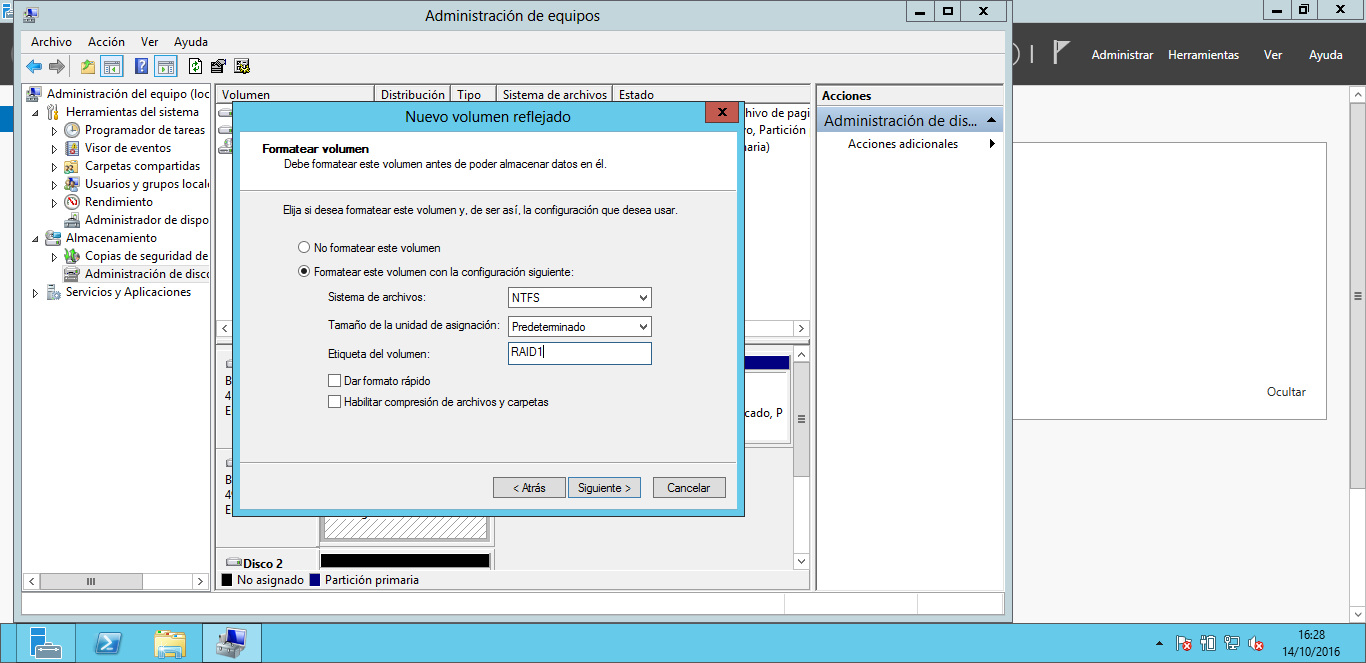
\includegraphics[width=0.9\textwidth]{raid1-6.png}
	\caption{Formateamos el volumen con el sistema de archivos que queramos y dándole un nombre en el campo de etiqueta.}
\end{figure}
	
\begin{figure}[H]
	\centering
	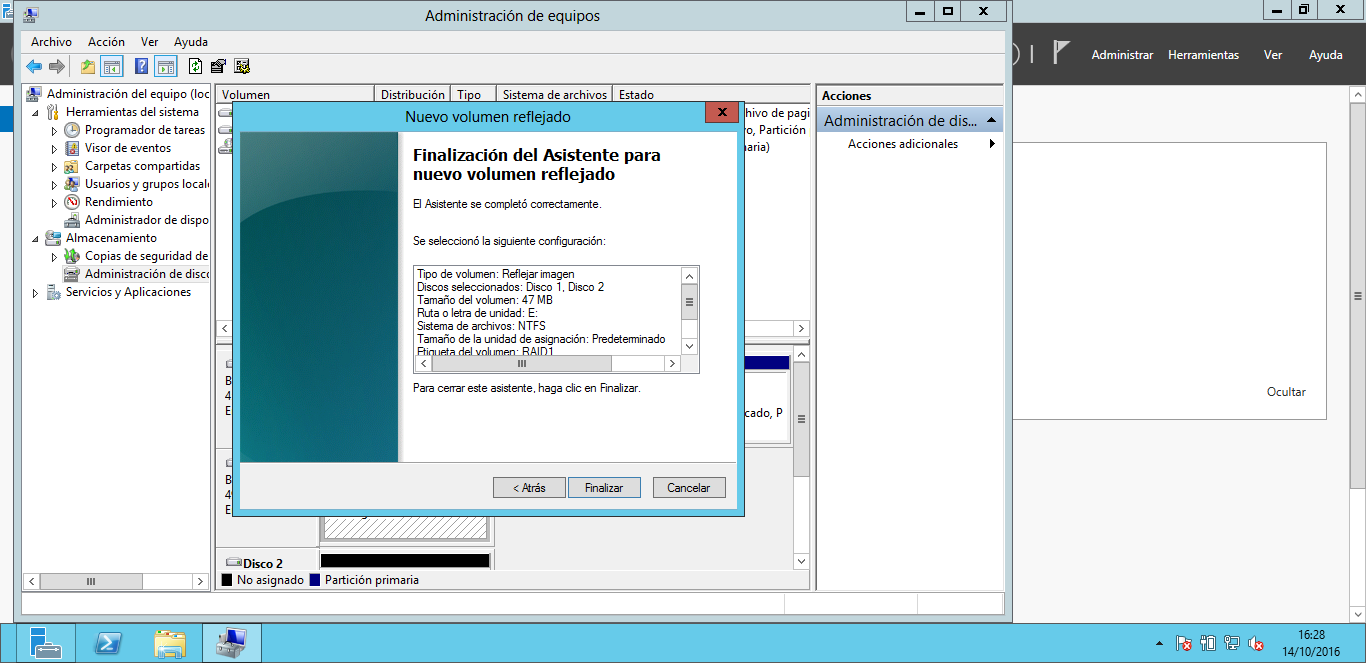
\includegraphics[width=0.9\textwidth]{raid1-7.png}
	\caption{Se nos mostrará un resumen y pulsamos finalizar.}
\end{figure}
\begin{figure}[H]
	\centering
	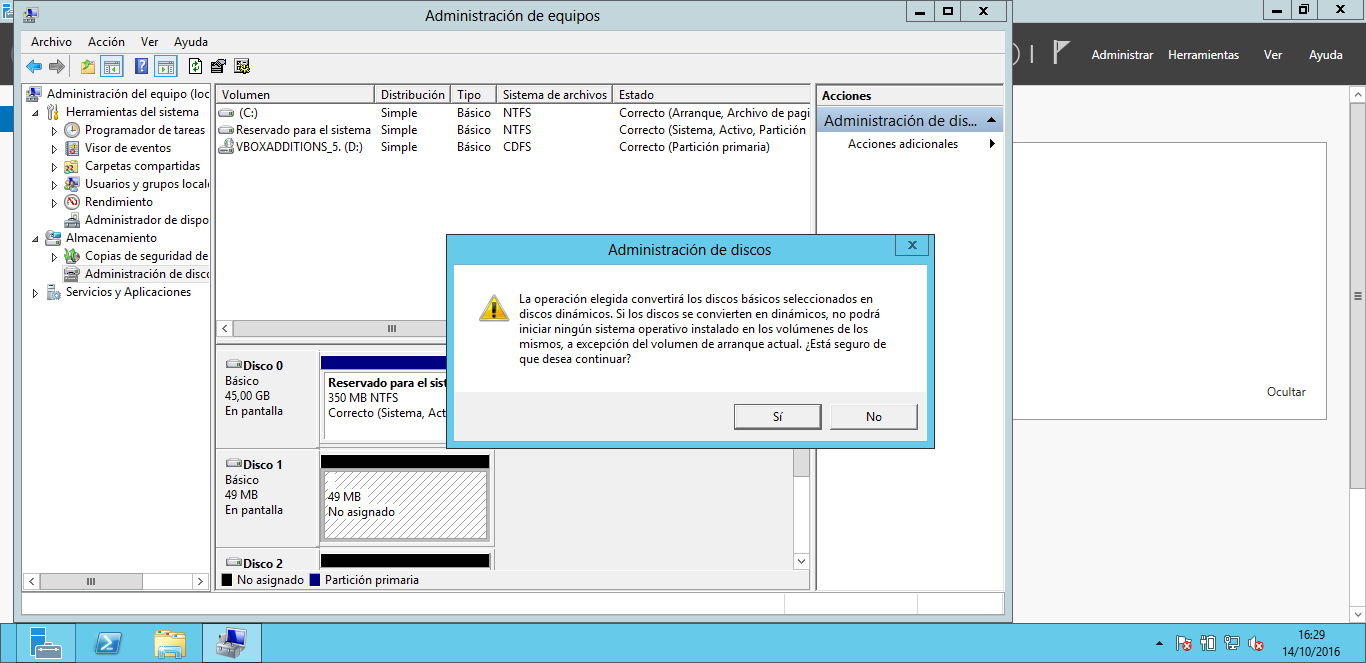
\includegraphics[width=0.9\textwidth]{raid1-8.png}
	\caption{Confirmamos que deseamos convertir los discos básicos en dinámicos.}
\end{figure}

%----------------------------------------------------------------------------------------
%	Cuestión 14
%----------------------------------------------------------------------------------------

\section{Explique brevemente qué diferencias hay entre los tipos de conexión que permite el VMSW para las Mvs: NAT, Host-only y Bridge}

\textit{Fuente para la respuesta \cite{c14}}

\subsection{NAT}
Utilizando NAT la máquina virtual actúa como si estuviese accediendo a través de un router, pero en realidad es el motor de red de VirtualBox el que actúa como tal. Debido a esto, a no ser que realicemos redireccionamiento de puertos para evitarlo la máquina virtual no será accesible desde Internet, lo cual puede interesarnos o no.

\subsection{Host-only}
Permite que las máquinas virtuales puedan conectarse entre ellas pero, a diferencia de Bridge, no simulan una conexión física al router y no tienen acceso a ninguna red exterior mas allá de la máquina host.

\subsection{Bridge}
En este caso VirtualBox instala un driver en el sistema operativo host que filtra el tráfico de las máquinas invitadas. Así externamente parecerá que la máquina está directamente conectada al punto de acceso, ya que a diferencia de en NAT recibirá una IP propia.

%------------------------------------------------

\bibliography{citas} %archivo citas.bib que contiene las entradas 
\bibliographystyle{ieeetr} % hay varias formas de citar

\end{document}
